\newpage
\null
\vspace{0.15cm}

\begin{center}
    \Huge{\textbf{\underline{Chapter 5: Deadlock}}}
\end{center}

\vspace{0.25cm}

\setcounter{section}{0}

\section{Processes \& Resources}
\begin{prettyBox}{S}{myblue}
Processes in an \textbf{(OS)} use various resources such as peripherals, variables, and files, following these steps:
\begin{enumerate}
    \item Request a resource, if it is unavailable the process is put on wait.
    \item Hold and use the resource.
    \item Release the resource once the operation is completed.
\end{enumerate}
\end{prettyBox}

\vspace{0.25cm}

\section{Deadlock}
\begin{prettyBox}{What is Deadlock?}{myblue}
Deadlock is a situation where a set of processes becomes blocked because each process is holding a resource and waiting for another resource held by another process to be released.
\end{prettyBox}

\vspace{0.15cm}

\section{Resource-Process Graph}
\begin{center}
    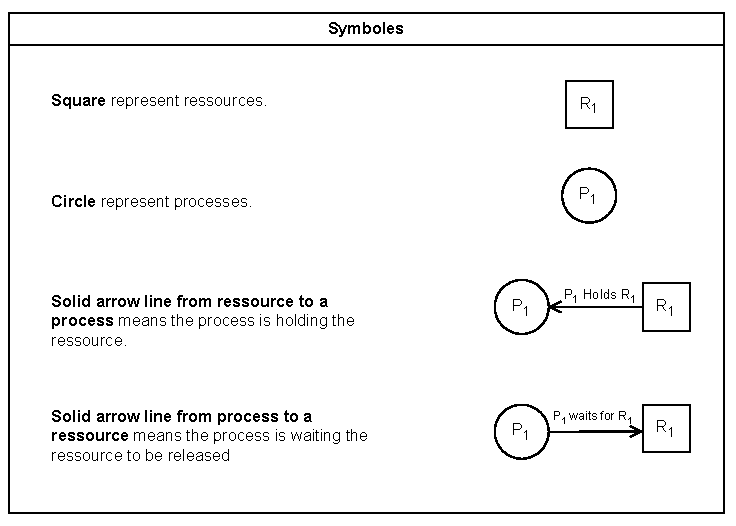
\includegraphics{Chapters/Diagram/Deadlock/sym.drawio.pdf}
\end{center}

\vspace{0.25cm}
\null
\section{Conditions for Deadlock}
\begin{prettyBox}{Coffman Conditions}{myblue}
Deadlock can arise if all the following conditions are met:
\begin{itemize}
    \item \textbf{Mutual Exclusion}: Only one process can hold a resource at a time.
    \item \textbf{Hold and Wait}: A process holding at least one resource is waiting for additional resources held by other processes.
    \item \textbf{No Preemption}: The \textbf{OS} cannot forcibly remove a resource from a process.
    \item \textbf{Circular Wait}: There is a cycle in the graph of two or more processes waiting for each other to release ressources.
\end{itemize}
\end{prettyBox}

\vspace{1cm}

\begin{center}
    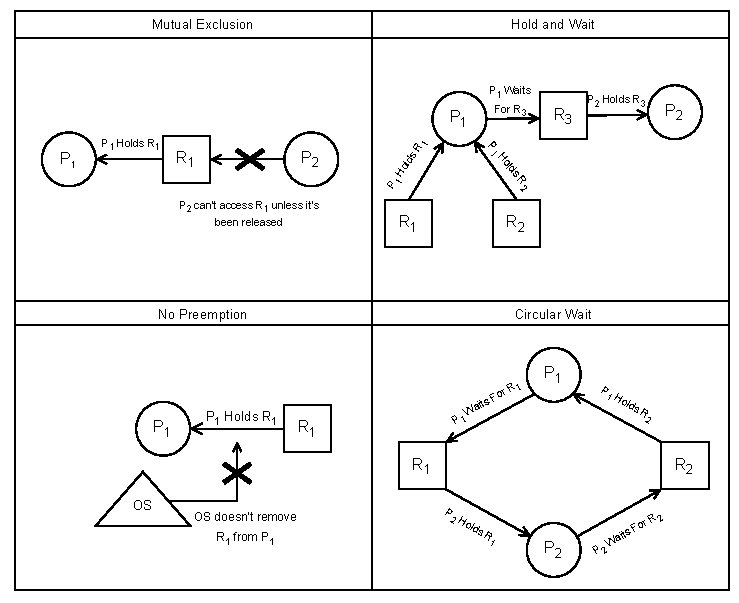
\includegraphics{Chapters/Diagram/Deadlock/coffman.drawio.pdf}
\end{center}

\newpage
\null
\section{Handling Deadlocks}
\begin{prettyBox}{Methods}{myblue}
\begin{itemize}
    \item \textbf{Ignore the Problem}: If resolving deadlocks is too costly, the \textbf{OS} may adopt a laissez-faire approach, ignoring deadlocks and requiring a system reboot if necessary.
    \item \textbf{Detection and Resolution}: The system detects deadlocks, often using algorithms like \textbf{DFS} on the resource allocation graph, and resolves them through one of the following strategies:
    \begin{itemize}
        \item \textbf{Preemption}: Reassign a resource from one process to another, which may lead to issues like inconsistency or lost progress.
        \item \textbf{Rollback}: Restore the system to a previously saved state and reallocate resources to avoid deadlock.
        \item \textbf{Termination}: Kill one or more processes involved in the deadlock to free resources.
    \end{itemize}
    
   \item \textbf{Avoidance}: Dynamically allocate resources in a way that avoids unsafe states, using the \textbf{Banker's Algorithm} to check the safety of each potential allocation before it is made.

    \item \textbf{Prevention}: Prevent deadlocks by ensuring at least one of Coffman’s conditions cannot occur:
    \begin{itemize}
        
\item \textbf{Mutual Exclusion}: Use serialized access (e.g., queues) to eliminate contention by ensuring resources are accessed in an orderly fashion. This doesn't remove mutual exclusion, but it allows the system to control priority, avoiding chaotic competition between processes.
        \item \textbf{Hold and Wait}: Require processes to request all the resources they need at the beginning. 
        While this prevents deadlocks, it can lead to inefficiency because resources may remain idle, and a resource may need to be released to be used by another.
        \item \textbf{No Preemption}: Allow preemption for certain resources by forcibly reallocating them. This
            approach is rarely practical due to the complexity of saving and restoring resource states.
        \item \textbf{Circular Wait}: Resources are assigned increasing numerical labels. Processes must request 
    resources in increasing order of their labels. If a process needs a previously allocated resource, it must first
    release any resources with higher labels before requesting the lower-numbered one. This ensures that no cycles can form in the resource allocation graph, preventing deadlock.
    \end{itemize}
\end{itemize}
\end{prettyBox}

